\documentclass[border=3pt]{standalone}
% Preâmbulo compartilhado pelos diagramas TikZ da aula 5 de IHC (Processos de Design)
\usepackage[T1]{fontenc}
\usepackage[utf8]{inputenc}
\usepackage{lmodern}
\usepackage{amsmath}
\usepackage{xcolor}
\usepackage{tikz}
\usetikzlibrary{arrows.meta,angles,quotes,decorations.pathmorphing,calc,
                positioning,shapes.geometric,shapes.misc,backgrounds,fit,
                math}

% Paleta (mesma dos SVGs originais)
% Paleta da disciplina de IHC: acento roxo (#755099), da capa do livro.
% (o nome "dblue" é mantido para não alterar todos os diagramas)
\definecolor{dblue}{HTML}{755099}
\definecolor{dorange}{HTML}{B3541E}
\definecolor{dgreen}{HTML}{4A7C59}
\definecolor{dred}{HTML}{9C4B4B}
\definecolor{dcream}{HTML}{F4F1EA}
\definecolor{dshade}{HTML}{DDD7C9}

% Função gaussiana (não normalizada por padrão de escala visual)
\pgfmathdeclarefunction{gauss}{3}{%
  \pgfmathparse{1/(#3*sqrt(2*pi))*exp(-((#1-#2)^2)/(2*#3^2))}%
}

% Estilos comuns (prefixo d... para não colidir com chaves internas do pgf)
\tikzset{
  >={Stealth[length=2mm]},
  dguide/.style={gray!55, dashed, line width=0.4pt},
  daxis/.style={gray!60, line width=0.7pt, ->},
  dbody/.style={fill=black!3, draw=black!80, line width=1pt},
  dacc/.style={draw=dblue, line width=1pt},
  dlbl/.style={black!55, font=\small},
  dsub/.style={black!45, font=\footnotesize},
  dstate/.style={circle, draw=black!80, fill=dcream, line width=1pt,
                 minimum size=17mm, font=\large, inner sep=1pt},
  dobs/.style={circle, draw=black!80, fill=dshade, line width=1pt,
               minimum size=14mm, font=\large, inner sep=1pt},
  dbox/.style={rounded corners=2pt, draw=black!80, fill=dcream, line width=1pt,
               align=center, inner sep=6pt},
  dop/.style={circle, draw=black!80, fill=white, line width=1pt,
              minimum size=6mm, inner sep=0pt, font=\small},
  dtrans/.style={->, dblue, line width=1pt},
  dmeas/.style={->, dorange, line width=1pt},
  dcurve/.style={line width=1pt, dblue},
  dcurveb/.style={line width=1.4pt, dorange},
}

\begin{document}
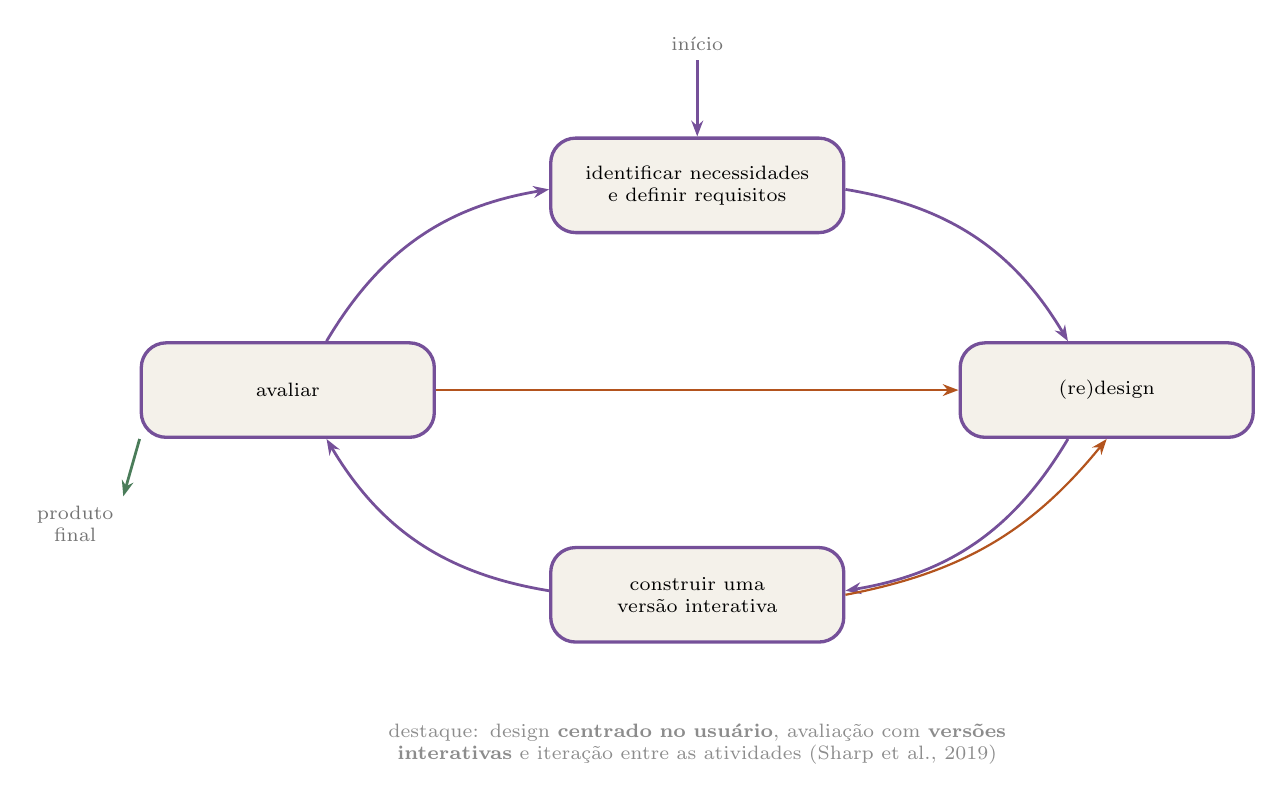
\begin{tikzpicture}[x=1cm,y=1cm,
   act/.style={dbox, rounded corners=9pt, text width=3.3cm, minimum height=1.2cm, font=\scriptsize, draw=dblue, line width=1.2pt}]

  \node[act] (id) at (0,3.4) {identificar necessidades e definir requisitos};
  \node[act] (rd) at (5.2,0.8) {(re)design};
  \node[act] (cv) at (0,-1.8) {construir uma versão interativa};
  \node[act] (av) at (-5.2,0.8) {avaliar};

  \node[dlbl, font=\scriptsize] (ini) at (0,5.2) {início};
  \draw[dtrans] (ini) -- (id);
  \draw[dtrans, bend left=25] (id) to (rd);
  \draw[dtrans, bend left=25] (rd) to (cv);
  \draw[dtrans, bend left=25] (cv) to (av);
  \draw[dtrans, bend left=25] (av) to (id);
  \draw[dmeas, line width=0.8pt] (av.east) -- (rd.west);
  \draw[dmeas, line width=0.8pt, bend right=20] (cv.east) to (rd.south);

  \node[dlbl, font=\scriptsize, align=center] (pf) at (-7.9,-0.9) {produto\\final};
  \draw[dtrans, dgreen] (av.south west) -- (pf.north east);

  \node[dsub, font=\scriptsize, align=center, text width=10cm] at (0,-3.7) {destaque: design \textbf{centrado no usuário}, avaliação com \textbf{versões interativas} e iteração entre as atividades (Sharp et al., 2019)};

\end{tikzpicture}
\end{document}
